% Asset ID: AS1CoordinateGeometryCirclesTikZ-007
% Purpose: Angle in a semicircle.
\documentclass[tikz,border=8pt]{standalone}
\usetikzlibrary{calc,angles,quotes}
\begin{document}
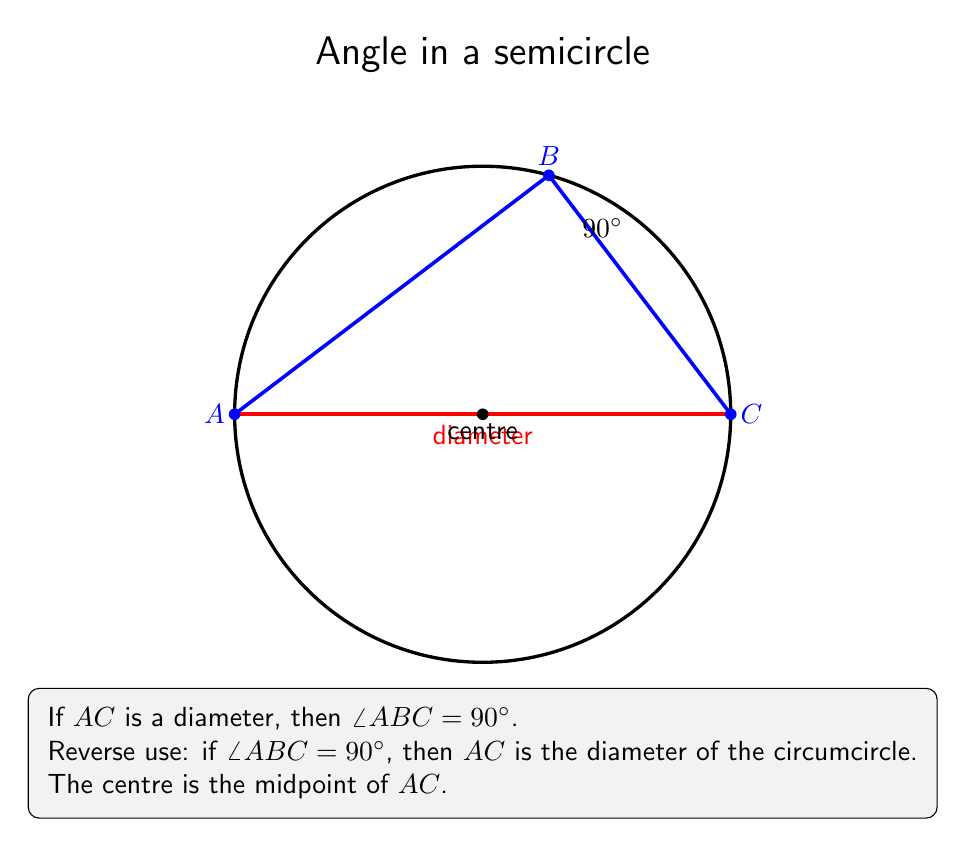
\begin{tikzpicture}[scale=1.05, font=\sffamily]
\node[align=center] at (0,4.35) {\Large Angle in a semicircle};
\coordinate (O) at (0,0); \draw[line width=1.2pt] (O) circle (3);
\coordinate (A) at (-3,0); \coordinate (C) at (3,0); \coordinate (B) at (0.8,2.89);
\draw[line width=1.3pt, red] (A)--(C) node[midway, below] {diameter}; \draw[line width=1.3pt, blue] (A)--(B)--(C);
\fill[blue] (A) circle (2pt) node[left] {$A$}; \fill[blue] (B) circle (2pt) node[above] {$B$}; \fill[blue] (C) circle (2pt) node[right] {$C$}; \fill[black] (O) circle (2pt) node[below] {centre};
\node at (1.45,2.25) {$90^\circ$};
\node[align=left, draw, rounded corners, fill=gray!10, inner sep=7pt] at (0,-4.1) {If $AC$ is a diameter, then $\angle ABC=90^\circ$.\\Reverse use: if $\angle ABC=90^\circ$, then $AC$ is the diameter of the circumcircle.\\The centre is the midpoint of $AC$.};
\end{tikzpicture}\end{document}
